\chapter{Introduction}
Water is a fundamental molecule that plays an important role  in driving
numerous biological, chemical, environmental, and industrial processes \cite{henry2005state,Kurz2008,ahuja2013green}. Water
is ubiquitous where it comprises two-thirds of earth and about half the volume of every living biological cell~\cite{Kontogeorgis2022,ling2004determines}.  Its unusual properties include  strong network
of hydrogen bonds which directly correlates to high boiling
point,	strong cohesion,
high surface
tension, heat of vaporization, and low vapor
pressure; ice has lower density than liquid water; and excellent solvent due to
its polar nature that
dissolve a wide range of substances, making it an excellent medium for chemical
reactions and biological processes \cite{Kontogeorgis2022,brini2017water}.

Due to its high cohesion, water can easily form surfaces and boundaries. Water
interfaces have important applications in heterogeneous catalysis \cite{fechete2012past}, fuel cells \cite{Owejan2009},
and protein folding \cite{levy2006water}. In particular, aqueous solution containing salts affects
electrochemical gradients  that have important role in	cell membrane
regulation \cite{lai2006distribution}. Despite extensive research on both experimental and theoretical fronts,
there exists a challenge in accurately modeling structural and dynamical
properties of salt solutions. An example is the role of electrolytic salt concentration in
affecting the surface tension of water as shown in
Figure~\ref{fig:surf_tens_solute}, where different trends are observed for
different chemical species. For instance, salts containing divalent cations have steeper upward slope  than monovalent cations. Moreover, the surface tension starts to plateau at higher concentration for some  salts such as \ch{NaBr}, \ch{KI}, \ch{NaI}, and \ch{NH_4Cl}.

Significant efforts were devoted to the development of models to reproduce the
behavior of water in computer simulations. The most
widely employed models for water are empirical models whose
parameters were obtained by fitting to experimentally measured properties \cite{Duin2001,brenner2002second,daw1984embedded}. While they provide a practical and efficient way to simulate large systems, empirical models are limited by their transferability to different chemical environments, their sensitivity to parameters used, rigidity since it assumes fixed bond lengths, angles, and dihedral angles based on equilibrium positions, and accuracy due to neglecting polarization and quantum effects. In contrast, \emph{ab initio} models are
determined from first principles and
therefore do not require fitting to experimental data \cite{car1985unified,Marx2009,kohn1965self}. However, \emph{ab initio} model is
computationally expensive since it requires to solve electronic structure problem at each molecular dynamics simulation step which greatly limits the  system size to few hundred atoms
and simulation timescale to few picoseconds. Nevertheless,
recent advances in machine learning (ML) have allowed the development of deep
neural network (DNN) potentials that
enables it to predict plethora of material properties  with the
same accuracy as the underlying \emph{ab initio} theory but as efficient as using
empirical methods \cite{Thompson2015,Huan2017,Behler2007,Behler2016,Chmiela2017,Unke2021}.
Machine learning methods aim to learn the functional relationship between inputs (chemical descriptors) and outputs (properties) from patterns or structure in the data which would ideally reflect  the underlying
effective ``rules'' of quantum mechanics \cite{schutt2020machine}.


This thesis will focus on the properties of a neat water (without any
solutes) in an interface and simulate relevant properties such as surface
tension, density, and dipole orientation using deep neural network potential
trained on bulk and with interfaces. Specifically, the objectives are

\begin{itemize}
    \item To develop accurate and transferrable DeepNN potentials for
          interfaces
    \item To explore the quality of the training data set in improving the
          description of water interfaces
    \item To understand reliability of the current architecture of DeepMD in
          dealing with interfaces
\end{itemize}

\begin{figure}[tbhp!]
    \centering
    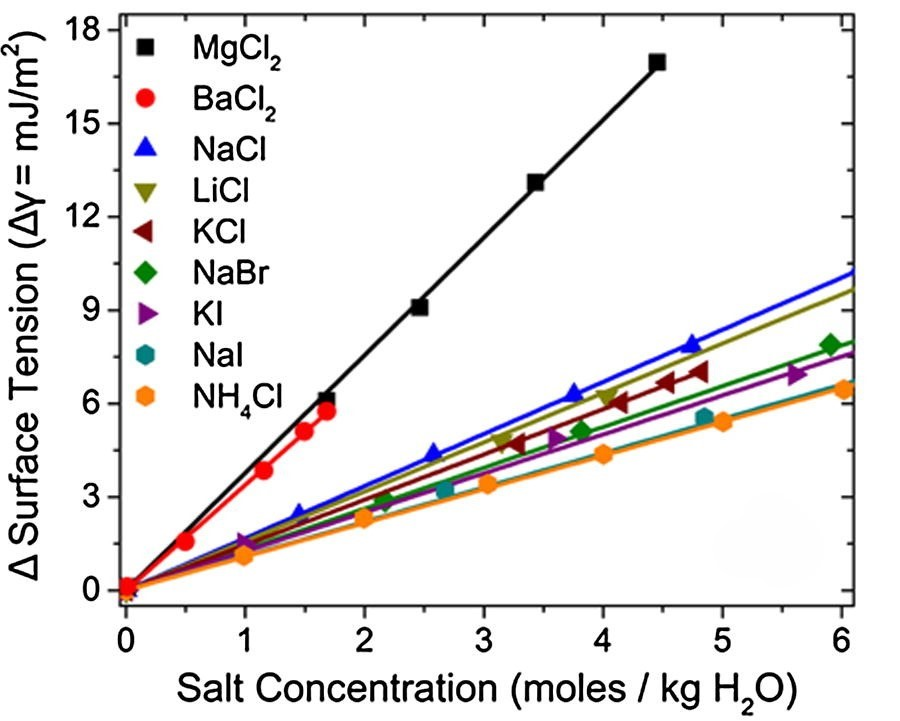
\includegraphics[width=0.7\linewidth]{images/ST_solute.jpg}
    \caption{Surface tension measurements of air/aqueous solution interfaces as a function of concentration for various salts. Image taken from \cite{okur2017jones}. }
    \label{fig:surf_tens_solute}
\end{figure}